\section{Déterminer un référentiel (4 points)}

\begin{center}
	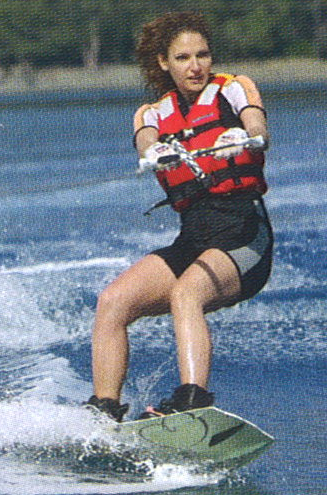
\includegraphics[scale=0.3]{board}
\end{center}

Un bateau se déplace sur un plan d'eau en ligne droite à une vitesse constante.
La wakeboardeuse, tractée par ce bateau a la même trajectoire.
\begin{questions}
	\question Déterminer dans quel référentiel la wakeboardeuse est :
	
	\begin{parts}
		\part[2] immobile
		\fillwithdottedlines{3cm}
		\part[2] en mouvement
		\fillwithdottedlines{3cm}
	\end{parts}
\end{questions}